\subsection{Bidirectional mapping through an example}
We present our additional constructs through a producer-consumer example, whose architecture is specified by Fig. \ref{fig:approachexample} \encircle{a}, \encircle{b}, and \encircle{c}.
The \ttt{p} producer sends data items to a first-in first-out component \ttt{FIFO} storing data for the consumer to pull it.
The data items are saved in a sized queue attribute, \ttt{queue}.
The latter is associated with the number of currently stored items (\ttt{numberOfItems}), the capacity (\ttt{MAX\_SIZE}), and other attributes and operations used for validating incoming items and the availability of the queue.
The \ti{pPush} port of the producer with \ttt{IPush} as required interface is connected to the \ti{pPush} port of \ti{FIFO} with \ttt{IPush} as provided interface. %so that the producer and FIFO can interact with each other through their respective port.
\ttt{FIFO} also provides the \ti{IPull} interface for the consumer to pull data items.
FIFO implements the two interfaces in Fig. \ref{fig:approachexample} \encircle{b}.

The behavior of \ttt{FIFO} is described by using a UML State Machine as in Fig. \ref{fig:approachexample} \encircle{c}.
Initially, the \ttt{Idle} state is active.
The state machine then waits for an item to come to the \ttt{fifo} component (through the \ttt{pPush} port).
The item is then checked for its validity.
The \ttt{DataQueuing} state verifies the availability of the queue to decide to either add the item to the queue or discard it.

Our additional constructs added to the existing programming language are categorized into structural and behavioral constructs.


\subsubsection{Structural constructs:}
Three constructs, \ti{Part}, \ti{Port}, and \ti{binding}, are introduced to represent UML \ti{part}, \ti{port}, and \ti{connector}, respectively, because these UML concepts do not have correspondences in the existing programming language.
Fig. \ref{fig:approachexample} \encircle{d} shows the intermediate code containing our additional constructs for the producer-consumer example.

In the intermediate code, the \ti{Part}s and \ti{Port}s constructs are template classes.
The template parameters of the latter specify the types of \ti{Part}s or required/provided interfaces of \ti{Port}s.
For example, lines 3-5 show the three parts corresponding to the ones defined in the model.
Lines 21 and 25 show ports with required interfaces and lines 29-30 show ports with provided interfaces.

UML connectors for communicating UML parts through UML ports are mapped to method calls (bindings) in the intermediate code.
Lines 7-8 shows two invocations to the \ti{bindPorts} function, which takes as input two ports (the two ports of the producer and fifo, for example).
Each class associated with a UML component contains a single configuration (as a method in lines 6-9) for port bindings.

Other model elements defined in the class diagram are mapped to the corresponding elements in the intermediate code.
For example, the UML operations and properties are mapped to the class methods and attributes (not shown in the paper), respectively; the UML interfaces (\ti{IPush} and \ti{IPull}) mapped to the classes with pure virtual methods (lines 11-18) (in C++). 

  

\begin{figure*}
	\centering
	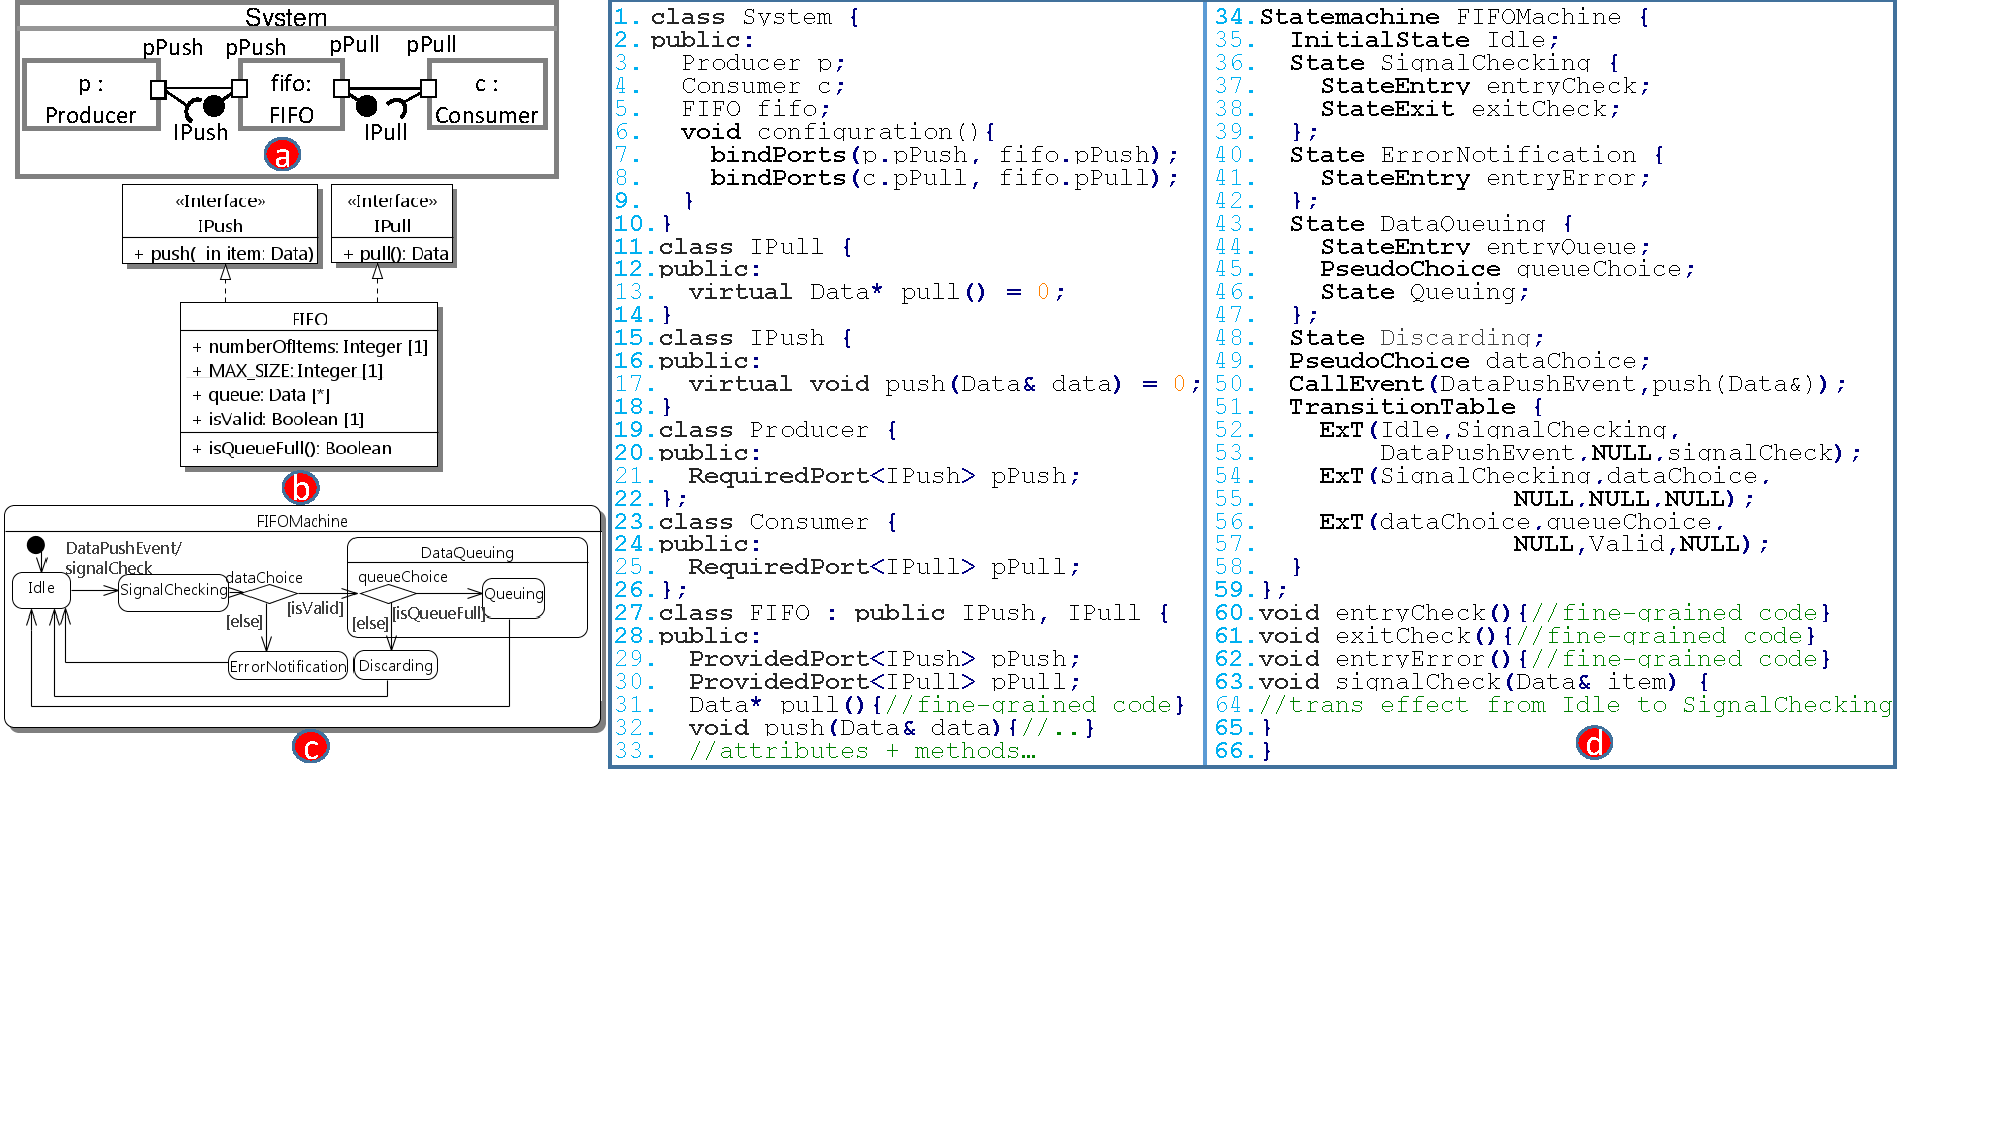
\includegraphics[clip, trim=0cm 5.9cm 1.6cm 0cm, width=\textwidth]{figures/approachexample.pdf}
	\caption{Architecture model and generated intermediate code} 
	\label{fig:approachexample}
\end{figure*}


\subsubsection{Behavioral constructs:}
%Applying XSeparation to UML State Machines, XSeparation-generated code contains our syntactic sugar of additional constructs for explicitly representing domain-specific concepts of state machines such as states and transitions.
These constructs are used to map to UML State Machine concepts.
The latter are divided into three sub-categories: vertex, event, and transition, which are specified into three parts: topology, events, and transition table in the intermediate code.


\noindent
\tb{Topology:}
A topology contains the constructs associated with UML vertexes to describe the state machine hierarchy.
In Fig. \ref{fig:approachexample}, the root of the topology is specified via the \ttt{StateMachine} keyword.
Other elements such as \ttt{region}, \ttt{state}, and \ttt{pseudo state} are hierarchically defined as sub-elements.
%Each element has a unique name.

State actions such as state entry/exit/doActivity are declared as attributes of the state.
These actions must be implemented in the owning class and has no parameter.
For example, \ttt{Idle} is an initial state. 
The \ttt{SignalChecking} state (lines 36-39) is declared with state actions, \ti{entryCheck} and \ti{exitCheck}. 
%The latter is specified as following: the entry/exit/doActivity action of a state, if declared within the topology, must be implemented as a method of the component/class. 
The \ti{FIFO} class implements the methods \ttt{entryCheck} and \ttt{exitCheck} (lines 60-61) for the state actions.
%The followings give the syntax of some elements in the generated code and the semantics mapped to the well-defined semantics in the UML specification \cite{OMG2015}.


Concurrent states with orthogonal regions in the intermediate code are not shown here due to space limitation. 
A State machine, state, or region in the intermediate code can declare pseudo states having similar syntax as attribute declarations of a class.
The type of pseudo state attributes is one of \ttt{\{PseudoEntryPoint, PseudoExitPoint, PseudoInitial, PseudJoin, PseudoFork, PseudoChoice, PseudoJunction, PseudoShallowHistory, PseudoDeepHistory, PseudoTerminate\}}, which correspond to the pseudo states defined in UML State Machine. 
%For example, \ttt{PseudoChoice dataChoice} and \ttt{PseudoChoice queueChoice} in Listing \ref{lst:fifostatemachine} represent the generated code for two \ttt{choice} pseudo states in the FIFO UML State Machine example.  

%\vskip 0.1cm
\noindent
\tb{Events:}
We support different constructs for four UML event types including \ttt{CallEvent}, \ttt{TimeEvent}, \ttt{SignalEvent}, and \ttt{ChangeEvent}.
The semantics of these events are clearly defined in the UML specification and beyond the paper's scope.

\begin{comment}
\begin{itemize}[\footnotesize]
	\itemsep0em
	\item A \ttt{SignalEvent} is associated with a signal type \ttt{sig}, whose data are described by attributes, and occurs if an instance of \ttt{sig} is received by a component through its data port by invoking \ttt{sendSignal} as previously discussed. 
	
	\item A \ttt{CallEvent} is associated with an operation \ttt{op} of the component class containing the state machine. 
	\ttt{CallEvent} is emitted if there is an invocation to \ttt{op}.
	
	\item A \ttt{TimeEvent} specifies the time of occurrence \ttt{dur} relative to a starting time. 
	The latter is specified as the time when a state, which accepts the time event, is entered.
	In other words, the state, which is the source vertex of a transition triggered by a time event, will remain active for a maximal amount of time specified by the time event.
	
	\item A \ttt{ChangeEvent} is associated with a boolean expression \ttt{expr}. 
	\ttt{ChangeEvent} is emitted if the value of \ttt{expr} changes from false to true.
\end{itemize}
\end{comment}

%The code generated by XSeparation for these events has syntax as followings:
\begin{comment}
\begin{itemize}[\footnotesize]
\itemsep0em
\item \ttt{CallEvent} $\rightarrow$ \tb{CallEvent} \tb{(} name\tb{,} op \tb{);}

\item \ttt{TimeEvent} $\rightarrow$ \tb{TimeEvent} \tb{(} name\tb{,} dur \tb{);}

\item \ttt{SignalEvent} $\rightarrow$ \tb{SignalEvent}<sig> name;

\item \ttt{ChangeEvent} $\rightarrow$ \tb{ChangeEvent} \tb{(} name\tb{,} expr \tb{);}
\end{itemize}

Essentially, each field in the syntax carries known semantics defined in the UML specification.
\begin{itemize}[\footnotesize]
\itemsep0em
\item \ttt{name} The unique identifier for an event.

\item \ttt{op} The name of the operation associated with a \ttt{CallEvent} and implemented in the active class. 

\item \ttt{dur} The duration associated with a \ttt{TimeEvent} and specified as millisecond.

\item \ttt{sig} The name of the signal class type (a UML signal is transformed into an object-oriented class) associated with a \ttt{SignalEvent}.
This signal type must be declared as required data of one of ports of the component in \tb{Component structure-prescribed code}.

\item \ttt{expr} The expression associated with a \ttt{ChangeEvent}. This expression is periodically evaluated to check whether its boolean value is changed.
\end{itemize}
\end{comment}

%\ttt{SimpleEvent} is a specialized \ttt{SignalEvent} without specifying an explicit signal.
%It is not explicitly standardized by UML but provided by tools such as QM \cite{qm} for practical reasons. 


%A \ttt{CallEvent} occurs if the method \ttt{method1} in the active class is called.
%\ttt{signal\_event(SE, Sig)}: A \ttt{SignalEvent} occurs if an instance of \ttt{Sig} is sent to the active class using its provided method \ttt{sendSig}.
%\ttt{time\_event(TE5ms, 5)}: A \ttt{TimeEvent} occurs after 5 millisecond from the moment the timer starts by entering some state.


%Call events are synchronous meaning that the processing runs within the thread calling the operation associated with a call event.
%Other events are asynchronous meaning that on receiving these events are stored in an event queue which is maintained at runtime for later processing.                                              
%A time event specifies the time of occurrence relative to a starting time. 
%The latter is specified when a state, which accepts the time event, is entered.
%The time event is emitted if the accepting state, which has at least one outgoing transitions triggered by the event, remains active longer that the relative time of occurrence. 	
%A change event has a boolean expression and is fired if the expression's value changes from false to true. 
%Note that not like call and signal events, time and change events are automatically fired inside the component.


%\vskip 0.1cm
\noindent
\tb{Transition table:}
It describes the transitions associated with UML transitions specified in the UM state machine at the model level. 
Three kinds of UML transitions, \ttt{external}, \ttt{local}, and \ttt{internal}, are supported but this paper only presents external transitions.
The difference between these kinds is clearly stated in UML and beyond the scope of this paper.

%For example, \ttt{CallEvent(DataPushEvent, push)} at line 23 in Listing \ref{lst:fifostatemachine} specifies that an event is fired whenever the \ttt{push} method, which is implemented by \ttt{FIFO} for the \ttt{IPush} interface provided by the \ttt{pPush} port, is invoked.
For example, line 50 shows a call event, which is emitted whenever there is an invocation the \ti{push} method if the FIFO class. 
The processing of the emitted event transitions from \ttt{Idle} to \ttt{SignalChecking} and executes the \ttt{signalCheckingEffect} transition method method associated with the transition if the current active state is \ttt{Idle}.
If so, the data item brought by the invocation will be checked for validity and further put to the queue or discarded.
Note that \ttt{signalCheckingEffect} has the same formal parameters with the \ttt{push} method.

%Code generated for a signal event has syntax as \tb{SignalEvent}\ttt{<sig> name}, in which \ttt{sig} is the name of the associated signal class (a UML signal is transformed into an object-oriented class).
%The signal type must be declared as required data of one of data ports of the component in \tb{Component structure-prescribed code}.
%Sending of a signal instance to the port might fire an asynchronous signal event for a state machine to handle in case that the containing component behavior of the port is specified via the state machine.
%Due to space limitation, we do not go to details of TimeEvent and ChangeEvent.

%\vskip 0.1cm
%\noindent
%\tb{Configuration:} 
%XSeparation-generated behavior code will be compiled to executable files by using our XSeparation compiler, which is presented in Section \ref{sec:compilation}.
%The executable files run in an asynchronous mode, in which according to UML State Machine, events, except CallEvent, are stored in an event queue at runtime.
 

%\vskip 0.1cm
\noindent
\tb{Deferred event:}
A state can declare \ttt{deferred events} using our additional construct \ttt{DeferredEvent}.
The deferred events are used for state machine execution to delay the processing of low-priority events when a certain state is active.
%The execution semantics of deferred events is that: given a current active state with declared deferred events and an event queue, the deferred events, if in front of the queue, will be moved to a deferred set and pushed back to the front of the queue once a non-deferred event is processed.
%In other words, the deferred events will not be processed while the state remains active.
